\documentclass[twoside, final, 11pt]{articleMine}
\usepackage[english]{babel} \usepackage{a4wide}
\usepackage{amsmath,amssymb,accents} \usepackage{epsfig}
\usepackage{subfigure} \usepackage{units} \usepackage{graphicx}
\usepackage[displaymath, mathlines, right]{lineno} \usepackage{xspace}
\usepackage{color} \usepackage{epic,eepic,pstricks}
\usepackage{acronym} \usepackage{wrapfig,multicol}
\usepackage{deluxetable} \usepackage{todonotes} 
\usepackage{hyperref}
\usepackage{float}
%\usepackage{slashbox}
\usepackage{lmodern} 
%\usepackage{caption}
\linenumbers
%\usepackage{showlabels}
\usepackage[draft]{showkeys}

%\usepackage[nolists, tablesfirst]{endfloat}
\graphicspath{{plots/}}
\newcommand*\patchAmsMathEnvironmentForLineno[1]{%
  \expandafter\let\csname old#1\expandafter\endcsname\csname #1\endcsname
  \expandafter\let\csname oldend#1\expandafter\endcsname\csname end#1\endcsname
  \renewenvironment{#1}%
     {\linenomath\csname old#1\endcsname}%
     {\csname oldend#1\endcsname\endlinenomath}}%
\newcommand*\patchBothAmsMathEnvironmentsForLineno[1]{%
  \patchAmsMathEnvironmentForLineno{#1}%
  \patchAmsMathEnvironmentForLineno{#1*}}%
\AtBeginDocument{%
\patchBothAmsMathEnvironmentsForLineno{equation}%
\patchBothAmsMathEnvironmentsForLineno{align}%
\patchBothAmsMathEnvironmentsForLineno{flalign}%
\patchBothAmsMathEnvironmentsForLineno{alignat}%
\patchBothAmsMathEnvironmentsForLineno{gather}%
\patchBothAmsMathEnvironmentsForLineno{multline}%
}
%\AtBeginFigures{\cleardoublepage}
%%%%%\parindent 5pt  
\parskip 1.2pt           % sets spacing between paragraphs
\def\Offline{\mbox{$\overline{\rm
Off}$\hspace{.05em}\raisebox{.4ex}{$\underline{\rm line}$}}\xspace}
\def\OfflineB{\mbox{$\bf\overline{\rm\bf
Off}$\hspace{.05em}\raisebox{.4ex}{$\bf\underline{\rm\bf line}$}}\xspace}

\def\eq#1{\begin{equation}#1\end{equation}}
%\def\al#1{\begin{align}#1\end{align}}
%\def\vc#1{{\bf #1}}
\def\pt#1{\accentset{\rightharpoonup}{#1}}
\include{myabbr}

\newcommand{\HRule}{\rule{\linewidth}{0.5mm}}
\newcommand{\VEM}{\mbox{VEM}}
\newcommand{\m}{\mbox{m}}

\let\stdsection\section  
%\renewcommand\section{\newpage\stdsection}  
 
\begin{document}

%\setpagewiselinenumbers
\modulolinenumbers[2]

%\linenumbers


\renewcommand\linenumberfont{\small\rmfamily}
\begin{center}
  \vspace*{-13ex}

  \rule{\linewidth}{0.1mm}  \\[17mm] {\huge  Matched filtering for EASIER data}
     \begin{flushright}
       \small 
     
     \end{flushright}

  % 
\end{center}
% 
\vspace*{2ex} 
%
\thispagestyle{empty}
\noindent
\begin{abstract}
  \noindent
We introduce in this note the method of matched filtering to EASIER data.
\end{abstract}

%
\thispagestyle{empty}
%$\;$
%\listoftodos
%\newpage
\noindent
%\section{Introduction}
The  IPN software  is inherited  from  a Karlsruhe  software that  was
adapted by Francesco for EASIER  and then modified by Olivier and Imen
to introduce their way to compute  the MBR signal. We aim at giving an
overview of the functionning of the software here. \\ 


\section{temperature measurement}
\label{sec:tempmeas}
We  describe  here  some  details  on  the  analysis  to  measure  the
temperature with the  sun flux. This analysis is  being carried out by
Corinne in Grenoble  and Romain in Paris. \\ The basic  idea is to use
the  monitoring data to  measure the  raise of  the baseline  upon the
passage of  the sun in the  field of view of  GIGADuck's antenna. This
raise  is used  to  estimate  the noise  temperature  of the  GIGADuck
system. The main steps of the analysis are:


\begin{figure}[!ht]
 \centering
 \hspace*{-3ex}
 \subfigure{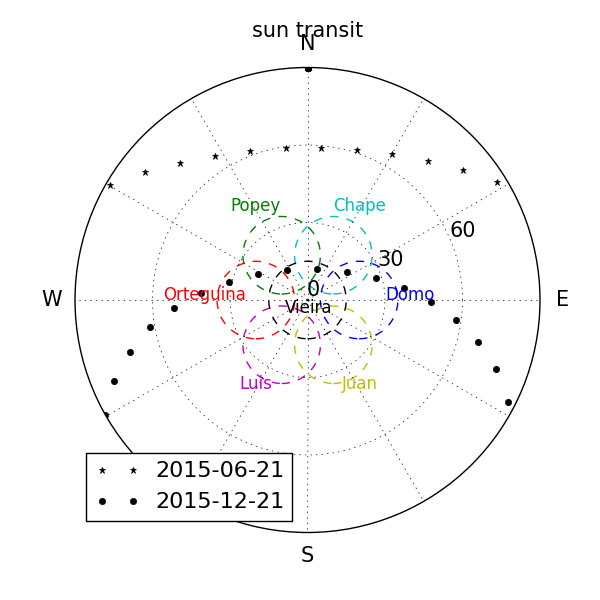
\includegraphics[width=0.49\linewidth]{sunpolar.png}}
 \subfigure{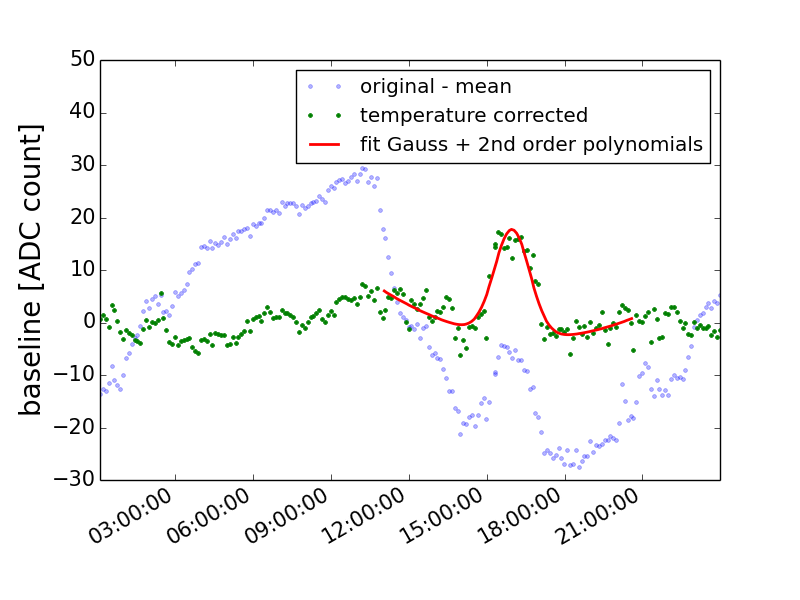
\includegraphics[width=0.49\linewidth]{examplesunfit.png}}
%% \subfigure{\includegraphics[width=0.49\linewidth]{sunexpected.png}}
 \caption{Left: Sun transit for the two solstices. The colored circles
   represent  the field  of  view of  the  GIGADuck antennas.   Right:
   Example  of the  baseline during  one  day. In  blue is  the
   orignal baseline when the mean is subtracted, in green after it was
   corrected from temperature dependence and  in red is a gaussian fit
   of to extract the signal from the sun.}
%%    Simulated  baseline  increase for  three  antennas  during the  sun
%%    passage.}
 \label{fig:sunsim}
\end{figure}


\begin{itemize}
\item produce the monitoring data
\item choose a period when the expected sun signal is large
\item cut the rainy periods
\item  find the  dependence of  the  radio baseline  with the  outside
  temperature during this period
\item correct the baseline for the outside temperature dependence
\item  fit the  radio baseline  with a  Gaussian plus  a  second order
  polynomial.
\end{itemize}




The figure~\ref{fig:sunsim} (left)  shows the path of the  sun for two
different dates and the field of  view of the GD C-band antennas.  The
sun signal  will be maximum  in summer when  the sun is higher  in the
sky.   The plot on  the right  in the  figure~\ref{fig:sunsim} (right)
shows the raw baseline of one antenna during one day in blue, the same
baseline corrected by  the tempereature dependence and the  fit of the
sun  bump in  red.  In  Corinne's  analysis, the  fit is  done with  a
constant  instead of  a  polynomials and  it  is done  on the  several
(around three)  consecutive days.  \\The  two methods have  shown very
similar  results.  They  show  differences between  antennas but  also
differences for  the same  antenna at different  time of the  year. We
intend in the next section  of this note to estimate the uncertainties
on this measurement to quantify the consistency of these results. 






\section{Temperature measurement uncertainties}
The formula we use to retrieve the temperature is:
\begin{equation}
  \rm
  T_{by's} (F_{sun}, A_{eff}, \Delta P) = \frac{\frac{1}{2} F_{sun} A_{eff}}{10^{\frac{\Delta P}{10}} -1 }
\label{eq:tsys}
\end{equation}
Where $\rm  F_{sun}$ is  the sun flux  measured by  other observatory,
$\rm A_{eff}$ is the effective area in the sun's direction, $\Delta P$
is the power difference in dB (with 1dB = 50 ADC count) and the factor
$\rm \frac{1}{2}$ is  the polarization factor (we only  observe one of
the two polarizations). The uncertainties on $\rm T_{sys}$ is then:
\begin{equation}
  \rm       \sigma_{T_{sys}}^2      =      \frac{T_{sys}^2}{F_{sun}^2}
  \sigma_{F_{sun}}^2  + \frac{T_{sys}^2}{A_{eff}^2} \sigma_{A_{eff}}^2
  +   T_{sys}^2   \bigg(\frac{   \frac{\ln(10)}{10}   10^{\frac{\Delta
        P}{10}}}{10^{\frac{\Delta P}{10}}  - 1}\bigg)^2 \sigma_{\Delta
    P}^2
\end{equation}

\subsection{Sun flux uncertainties}
Here we check the precision we have on the sun flux. Up to now, we get
data  at \unit[2.8]{GHz}  (commonly called  f107) and  extrapolate the
value at  \unit[3.8]{GHz} with parameterisation  of the quiet  sun and
the slowly varying  sun. We can compare our  results with the Nobeyama
observatory data, which  collects data on the sun  flux at \unit[2 and
  4]{GHz} (we don't use their data yet because they don't release them
on the web). The figure~\ref{fig:sunflux} shows different fluxes: 

\begin{figure}[!ht]
 \centering
 \hspace*{-3ex}
 \subfigure{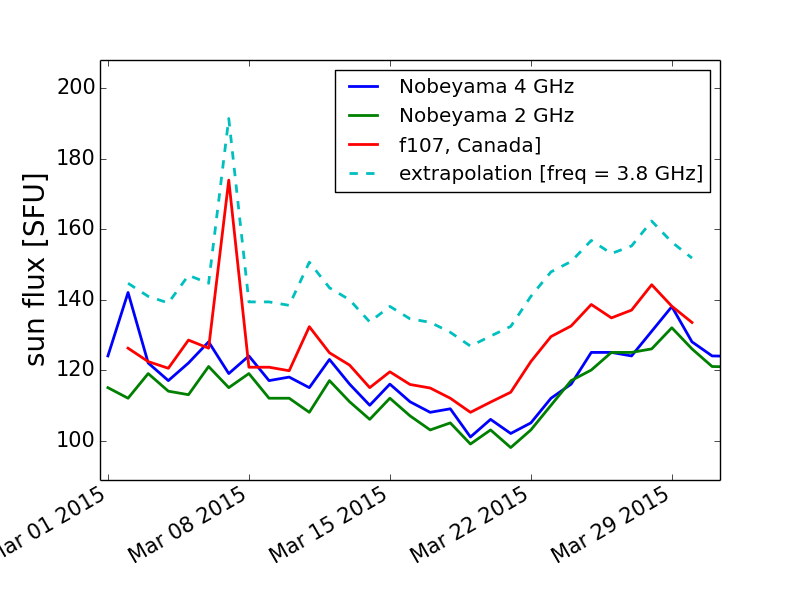
\includegraphics[width=0.49\linewidth]{sunfluxmarch.png}}
 \subfigure{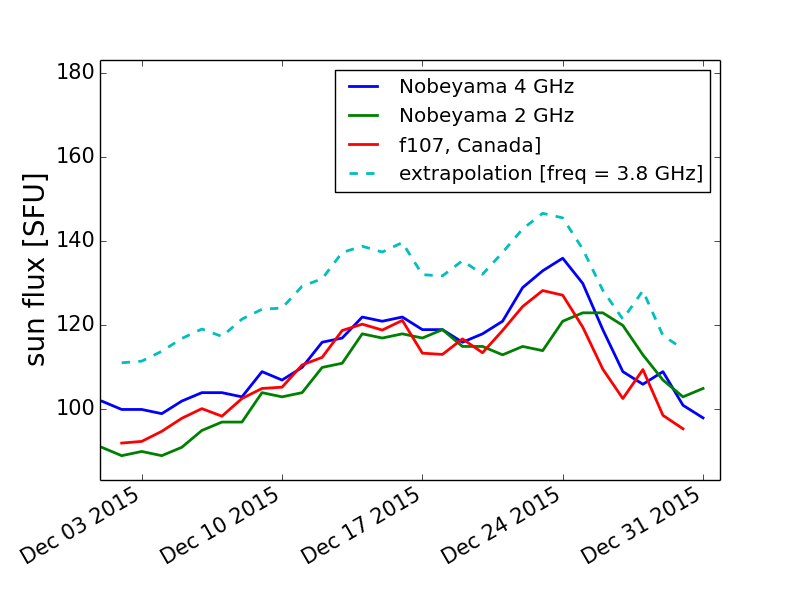
\includegraphics[width=0.49\linewidth]{sunfluxdec.png}}
%% \subfigure{\includegraphics[width=0.49\linewidth]{sunexpected.png}}
 \caption{sun flux for at different frequencies}
%%    Simulated  baseline  increase for  three  antennas  during the  sun
%%    passage.}
 \label{fig:sunflux}
\end{figure}
The value reported on the plots for the Nobeyama observatory are taken
from what is  displayed on their daily curves. I  don't really know if
this is an  average or the minimum value.  In any  case, the values at
\unit[2 and  4]{GHz} are lower than  what is measured  at the Canadian
site~\cite{sundata,  sundata2} by around  20\%. Since  I am  still not
sure of the meaning of the value for the Nobeyama data, I will account
for   an  uncertainty   of   20\%  in   the  temperature   calculation
(\textbf{this has to be improved either by taking the data of Nobeyama
  or  by determining  a precise  uncertainty.}). This  number  of 20\%
corresponds also to what is given in the website~\cite{sunparam} where
we found the parameterisation.


\subsection{Effective area uncertainties}
We  do have  also  some uncertainties  on  the effective  area, be  it
because of  the pointing  direction or our  knowledge of the  gain. We
estimate  the possible  shift  in pointing  to  2$\rm ^{\circ}$.   The
resulting uncertainty on  the gain depends on the  zenith angle at the
sun maximum.  The figure~\ref{fig:aeffuncert} shows the effective area
and  a  Gaussian  fit as  a  function  of  the  zenith angle  and  the
uncertainties on the effective area based of the Gaussian fit. 

\begin{figure}[!ht]
 \centering
 \hspace*{-3ex}
 \subfigure{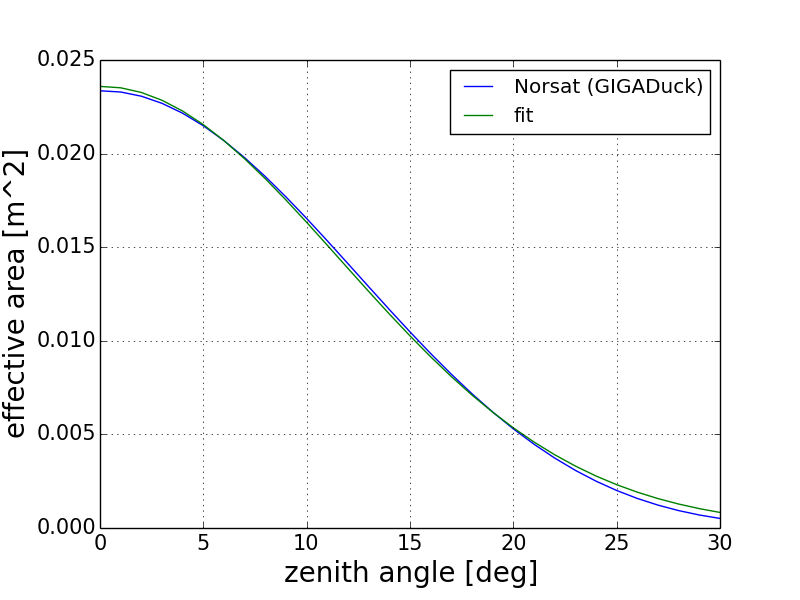
\includegraphics[width=0.49\linewidth]{aeff.png}}
 \subfigure{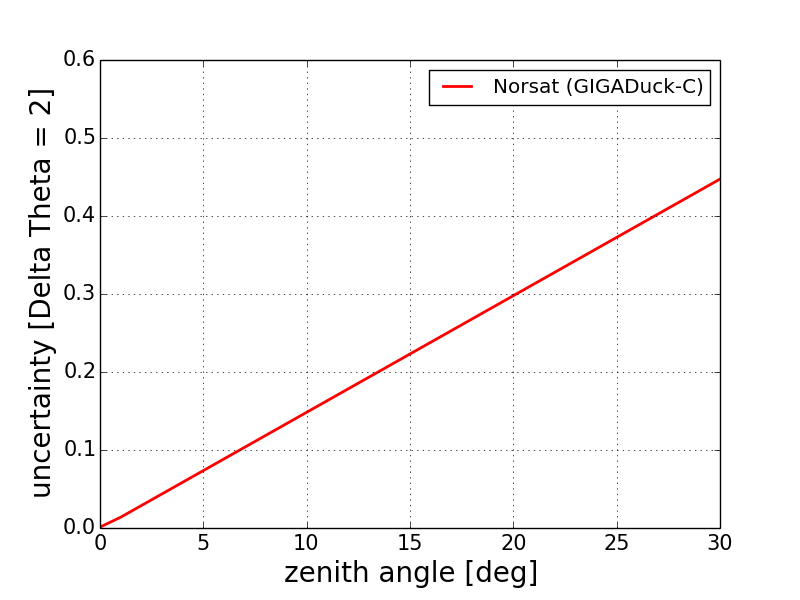
\includegraphics[width=0.49\linewidth]{sigmaaeff.png}}
 \caption{Effective  area of  the AInfo  antenna from  HFSS simulation
   (blue), Gaussian  fit (green).  Right: relative uncertainty  on the
   effective area}
 \label{fig:aeffuncert}
\end{figure}
We perform the  temperature measurement only during the  months when a
significant signal  from the  sun is expected,  that means when  it is
high in the  sky. The zenith angle at which the  sun signal is maximum
(in the simulation) is  shown in the figure~]\ref{fig:zenithofmax} for
  three antenna:  Vieira the  central detector that  points up  to the
  zenith, Chape  and Orteguina (see  figure~\ref{fig:sunsim} for their
  field of view).
\begin{figure}[!ht]
 \centering
 \hspace*{-3ex}
 \subfigure{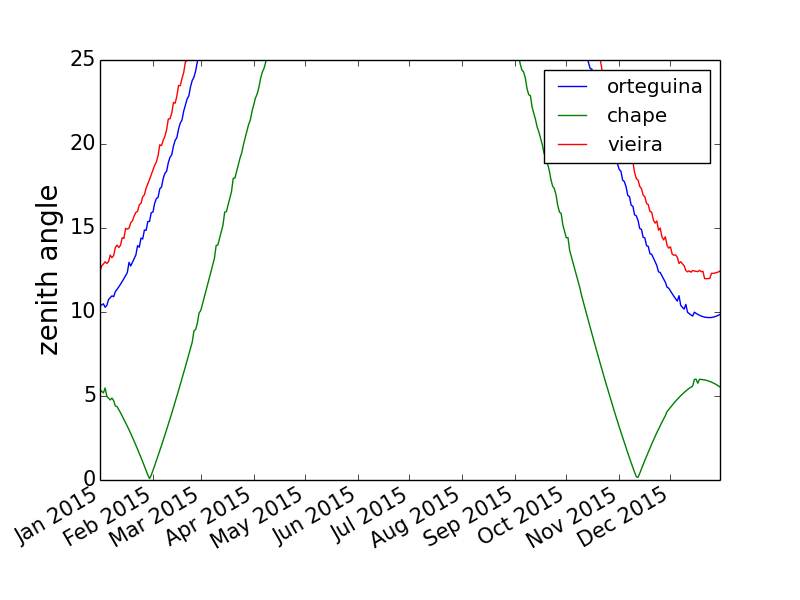
\includegraphics[width=0.49\linewidth]{zenithofmax.png}}
 \caption{Zenith angle when the sun signal is maximum as a function of
   the date}
 \label{fig:zenithofmax}
\end{figure}
The angle at  which the sun is observed when the  signal is maximum is
below  \unit[10]{$\rm  ^{\circ}$} for  Chape  but  around \unit[15  to
  20]{$\rm ^{\circ}$} in March for Vieira or Orteguina.


\subsection{Uncertainty on $\rm \Delta P$}
The uncertainty  on the measured power  induced by the  sun flux comes
from our  ability to measure a  variation of baseline on  an hour time
scale.   The  process  to   estimate  this  variation,  summed  up  in
section~\ref{sec:tempmeas}, is based  on a fit of the  sun bump with a
Gaussian function and the background with a second order polynominals.
There  aren't actually any  justification for  the background  fit. To
estimate the  error on  the $\rm  \Delta ADC$ we  make, we  change the
fitting   method    and   see    how   the   results    change.    The
figure~\ref{fig:fits}  shows the  results  of $\rm  \Delta  ADC$ as  a
function  of  the date  when  the baseline  is  either  fitted with  a
constant  and a  Gaussian  or with  a  second order  polynomial and  a
constant, on  the right side  is shown the corresponding  histogram of
the difference of the two methods. 

%%\section{Description}
lalalala

%%\include{conclusion/conclusion}

\addcontentsline{toc}{chapter}{Bibliography}                                 
\bibliographystyle{atlasnote}
\bibliography{thebib}
%% \newpage

\end{document}
